\section{Network, Data and Battery Models}
\label{ch1:sec:data-and-network-models}

All key network parameters and their associated cost functions have now been established.
In this section the network model and power flow simulation, from which all aforementioned key network parameters were extracted is explained.
Also, all data that is used throughout the research, as it is presented in this chapter, is included presented, too.

\subsection{Standardised Network Model}
\label{ch1:subsec:standardised-network-model}

The IEEE Power and Energy Society (IEEE-PES) provided several multi-node test feeder cases.
These test cases used to be limited to distribution networks in the United States.
In 2015 however, they published a standardised model of a LV distribution network for the UK power network.
This model is called the ``European Low Voltage Test Feeder'' and an OpenDSS compatible version can be obtained from their website, too \cite{DistributionTestFeeders2017}.
Within the context of this work, the feeder is referred to as the ``LV Test Case'' and a network plot of this feeder has been included for reference.

\begin{figure}\centering
	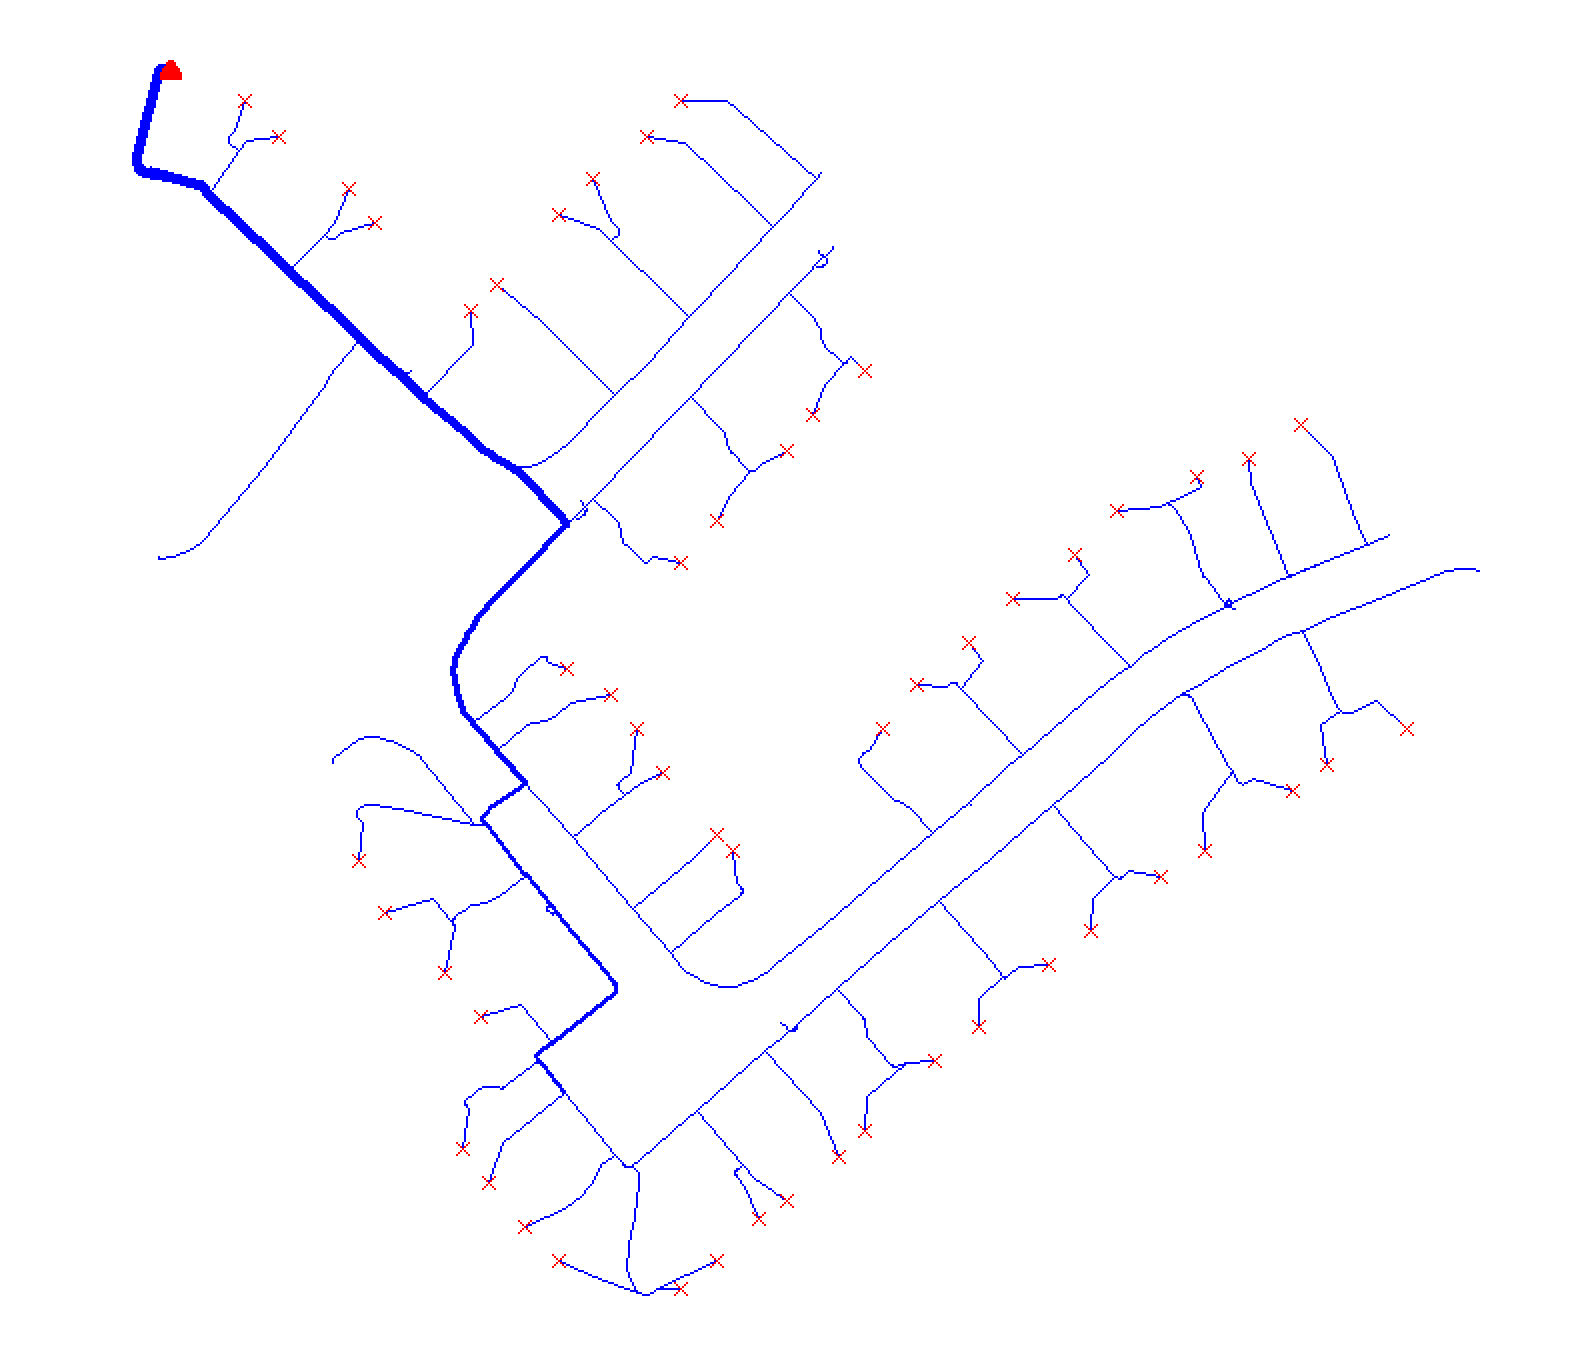
\includegraphics[width=0.8\textwidth]{_chapter1/fig/network-plot-LVTestCase}
	\caption{A power flow plot of the IEEE-PES European Test Case Feeder, i.e. a LV distribution network in the UK.}
	\label{ch1:fig:network-plot-LVTestCase}
\end{figure}

Here, a substation (triangle in north west) provides power to the feeder, and the amount of power is visualised by using a thicker line plot.
There are 55 single-phase households connected to the substation and for this particularly case, are each customer drew 2kW.

\subsection{Load Profiles: Minutely and Half-Hourly}

Alongside the LV Test Case, 100 minutely demand profiles were supplied; each being 24h long.
A series of 1440 snapshot simulations was run, by assigning one load profile to one customer.
Doing so made it possible to simulate the variation and volatility in demand over a day.
Since the values given are active power values, a standardised power factor of 95\% was used for all loads.
This non-unity power factor simulates a certain inductive load, which would otherwise be neglected.

Since the minutely profiles' resolution is too high in order to effectively calculate battery schedules, they had to be down-sampled.
This down-sampling was achieved by first calculating the daily demand profile at sub-half-hourly resolution.
Then, the day was split into 48 half-hourly time-slots, and the average power was computed for each.

\subsection{Battery Model}
